\documentclass{apuntes}

\title{Aprendizaje Automático}
\author{Víctor de Juan}
\date{15/16 C1}
\usepackage{bm}
% Paquetes adicionales

% --------------------




\begin{document}
\pagestyle{plain}
\maketitle

\tableofcontents
\newpage
% Contenido.

\chapter{Introducción}


Aristóteles en el siglo IV a.c. dice que el razonamiento deductivo se analiza aplicando 2 silogismos fuertes.

\begin{defn}[Silogismos fuertes] Premisa:  $A \implies B$
\begin{itemize}
\item[1] Si observamos A, deducimos B.
\item[2] Si observamos $\neg B$, deducimos que $\neg A$.
\end{itemize}
\end{defn}

\begin{defn}[Silogismos débiles] 
Si vemos la calle mojada, $\implies$ lo más probable es que haya llovido.
\end{defn}


\section{Introducción a la probabilidad}

Vamos a repasar conceptos de probabilidad para poder utilizar los silogismos débiles.

\begin{defn}[dominio]
Todos los posibles resultados de un experimento aleatorio.
\end{defn}

\begin{defn}[Variable aleatoria]
Variable que identifica el experimento aleatorio
\end{defn}

\begin{defn}[Suceso]
Valor que toma la variable aleatoria al realizar el experimento aleatorio.
\end{defn}

\paragraph{Ejemplo:} Tirar un dado.

\begin{itemize}
	\item Dominio $= \{1,2,3,4,5,6\}$
	\item Variable $X$ representa tirar un dado.
	\item Posibles sucesos: $X=1,X=2,...,X=6$
\end{itemize}

A partir de esto ya podemos calcular probabilidades: 

$$P\left(primo\right)$$

$$P\left(par\right)$$



Más repaso de probabilidad: probabilidad condicionada (regla de la suma) 

\begin{defn}[Regla del producto]
\[P(A,B|I) = P(A|B,I) · P(B|I) = P(B|A,I) · P(A|I)\]
\end{defn}

Vamos a ver cómo utilizar esta regla combinándola con los silogismos:

Podemos incluir el primer silogismo fuerte \ref{silogismofuerte} haciendo $I= A\implies B$, entonces tenemos:
\[P(A,B|A\implies B) = ... = 1\]
Y aplicando el segundo silogismo fuerte, tenemos:
\[P(A|\bar{B}, A\implies B) = ... = 0\]

Sin embargo, utilizando los silogismos débiles:

\[ P(A|B,A\implies B) = \frac{P(A|A\implies B)}{P(B|A\implies B)} \geq P(A|A\implies B)\]


\section{Toma de decisiones}

A la hora de tomar decisiones, podemos utilizar 2 criterios. El criterio de máxima verosimilitud y el de ...


\begin{defn}[Criterio MAP]
\label{CriterioMAP}
Maximiza la probabilidad a posteriori.

\[H_i = \max_i\{p(H_i | D)\} = \max_i \{\frac{P(D|H_i)·P(H_i)}{P(D)}\} = \max_i \{P(D|H_i)·P(H_i)\}\]

Donde $\max_i$ devuelve la hipótesis en la que se encuentra el máximo.
\end{defn}

\begin{defn}[Criterio MV]
\label{CriterioMV}
Maximiza la máxima verosimilitud.
\[
H_i = \max_i\{P(D|H_i)\}
\]

\end{defn}

La diferencia entre los 2 criterios es la corrección y por tanto la complejidad. \textbf{MAP es más correcto}, pero \textbf{MV} es \textbf{más fácil.} 

Vamos a verlo con un ejemplo.

\begin{example}
Tenemos monedas justas y monedas trucadas. Las monedas trucadas tienen un 75\% de salir cara.

Hemos obtenido cara en un lanzamiento. ¿Cuál es la probabilidad de que sea una moneda justa?

$D=c, H=t|j$

\[
P(j|c) = \frac{P(c|j)·P(j)}{P(c)} = \frac{0.5·0.5}{P(c)}
\]
\[
P(t|c) = \frac{P(c|t)·P(j)}{P(c)} = \frac{0.75·0.5}{P(c)}
\]

Como $P(j|c) + P(t|c) = 1$, tenemos que $P(c) = 0.5·0.5 + 0.75·0.5 = 0.625$, entonces:

\label{calculadoAnteriomente1}
\[P(j|c) = 0.4\]
\[P(t|c) = 0.6\]

Según el criterio MAP diríamos que es más probable que la moneda esté trucada. 

Por algún motivo, calculamos:

\[P(j|x) = \frac{P(x|j)·P(j)}{P(x)} = \frac{0.5·0.5}{P(x)} = \frac{0.25}{P(x)}\]
\[P(t|x) = \frac{P(x|t)·P(t)}{P(x)} = \frac{0.25·0.5}{P(x)} = \frac{0.125}{P(x)}\]

Normalizando obtenemos:
\label{calculadoAnteriomente2}
\[P(j|x) = \frac{2}{3}\]
\[P(t|x) = \frac{1}{3}\]

\subsection{Tasas de error}

Vamos a estudiar las tasas de error siguiendo con el ejemplo de las monedas.

\paragraph{Existen 4 modelos posibles:}
Tenemos:
\begin{itemize}
\item Espacio de atributos = $\{c,x\}$\footnote{cara o cruz}
\item Clases posibles\footnote{Clases que puede asignar nuestra hipótesis H} = $H\in\{j,t\}$
\end{itemize}

Vamos a construir los 4 modelos posibles:

\begin{itemize}
	\item $h_1(c) = j$ y $h_1(x) = t$ 
	\item $h_2(c) = t$ y $h_2(x) = j$ 
	\item $h_3(c) = j$ y $h_3(x) = j$ 
	\item $h_4(c) = t$ y $h_4(x) = t$ 
\end{itemize}

Con lo calculado anteriormente (\ref{calculadoAnteriomente1} y \ref{calculadoAnteriomente2}), observamos que el modelo $h_2$ es elegido según el criterio MAP. 

Pero podemos plantearnos, ¿qué modelo es mejor? Pues el que menos se equivoque. Vamos entonces a calcular las probabilidades de error de los modelos.

\textcolor{red}{Dejuan ha hecho a mano estos cálculos porque no tenía ni pies ni cabeza lo que había copiado.}

\paragraph{Cálculo de errores}
\subparagraph{$h_1$:} $P(error) = p(t,c) + p(j,x) = P(j|c)·P(c) + P(j|x)·P(x) = ... = 50\% $
También podíamos haber calculado (como estaba mal escrito en la versión anterior de los apuntes). A gusto del consumidor un método o el otro.
\[P(error) = 1-P(acierto) = 1 - (p(j,c) + p(t,x)) = ...\]

\subparagraph{$h_2$:} 
$P(error) = p(j,c) + p(t,x) = P(j|c)·P(c) + P(t|x)·P(x) = ... = 50\%$
\subparagraph{$h_3$:} 
$P(error) = p(t,c) + p(t,x) = P(t|c)·P(c) + P(t|x)·P(x) = ... = 62.5\%$
\subparagraph{$h_4$:} 
$P(error) = p(j,c) + p(j,x) = P(j|c)·P(c) + P(j|x)·P(x) = ... = 37.5\%$
\end{example}


 \begin{defn}[Matriz de confusión]
 	Tabla para visualizar el error de un clasificador. En la diagonal encontramos las tasas de acierto, y fuera de la diagonal, las tasas de error.
 \end{defn}


En esta matriz, la diagonal son las tasas de acierto y lo que está fuera de la diagonal las tasas de fallo. Con este criterio, comprobamos entonces que efectivamente la tasa de error es $25+12.5 = 37.5$, como habíamos calculado anteriormente erróneamente.


Si tomamos $h_2$, la matriz de confusión sería (tomando la parte real arriba y las predicciones a la izquierda):
\[
\begin{pmatrix}{ccc}
& justa & trucada \\\hline
j&A_{11}&A_{12}\\
t& A_{21}&A_{22}
\end{pmatrix}
\]
Y vamos a ir calculando cada $A_{ij}$.

¿CUál es la probabilidad de que digamos justa siendo la moneda justa? Para ello pensamos ¿Cuándo decimos nosotros justa? Cuando ha salido una cruz, entonces $A_{11}$ es la probabilidad de que sea justa y de que haya salido cruz, es decir $A_{11} = P(x,j) = P(x|j)·P(j) = P(j|x)·P(x)$. Entonces:

\[
\begin{pmatrix}{ccc}
& justa & trucada \\\hline
j& P(x,j) & P(x,t)\\
t& P(c,j) & P(c,t)
\end{pmatrix}
\]




\paragraph{Pero...}

Pensemos en el caso de una enfermedad y queremos, a partir de unos datos predecir si va a tener la enfermedad o no. Tenemos una enfermedad muy grave que padecen $10$ personas en una muestra de $15000$. Un modelo que diga que nadie la tiene, sólo falla en un $\frac{10}{150000} \sim 0$, un error muy bajo. ¿Es este modelo bueno? En casos como este, interesa saber detectar la enfermedad cuando se da y es un error mucho más grave no diagnosticar la enfermedad cuando sí la tiene, que diagnosticarla cuando no la tiene, con lo que, la matriz de confusión ya no es una buena manera de valorar modelos. Por ello construimos la matriz de coste o riesgo.

\begin{defn}[Matriz de coste (o riesgo)]
	Una matriz de coste o riesgo consiste en definir ponderaciones para la gravedad de cada uno de los tipos de error. 
\end{defn}


\paragraph{Regla simétrica vs Regla asimétrica}
 La \concept{Regla de Bayes simétrica} utiliza una matriz de coste que es igual que la matriz de confusión, es decir, la importancia de los errores es simétrica.  Por consiguiente, el lector avispado podrá imaginarse que la \concept{Relga de Bayes asimétrica} utiliza una matriz de costes distinta de la de confusión, es decir, la importancia de los errores no es simétrica.

 En el caso de la enfermedad descrito anteriormente, convendría utilizar una regla asimétrica. 

 \begin{example}
Vamos a ver un ejemplo de costes con el caso de las monedas. 

Sea $R$ el coste si pasamos una trucada por justa y $R'$ el coste si pasamos una justa por trucada.

En el caso de las monedas, suponemos $R = 3R'$, con lo que el cálculo de los costes quedaría así:


\subparagraph{$h_1$:} $P(error) = R' · P(j,c) + R · P(t,x) = ... = R' · 0.625$
\subparagraph{$h_2$:} $P(error) = R' · P(j,x) + R · P(t,c) = ... = R' · 1.37$
\subparagraph{$h_3$:} $P(error) = R' · P(j,x) + R · P(t,x) = ... = R' · 1.5$
\subparagraph{$h_4$:} $P(error) = R' · P(j,c) + R · P(t,c) = ... = R' · 0.5$

Entonces, es $h_4$ la hipótesis que minimiza el coste (con la ponderación elegida), aunque no es la que minimiza el error en términos generales (como hemos visto antes).

 \end{example}



\begin{problem}[lentillas]

Este es un ejemplo de problema multidimensional.

Aquí tenemos los datos de donde sacar las probabilidades:

\begin{tabular}{c|c|c|c|c}
\textbf{EDAD} & \textbf{LESIÓN} & \textbf{ASTIGM.} & \textbf{PROD\_LAGRIM} & \textbf{DIAGNOSTICO}\\\hline
joven & miopía & no & reducida & no \\
joven & miopía & no & normal & blandas \\

joven & miopía & sí & reducida & no \\
joven & miopía & no & normal & duras \\

joven & hipermetropía & no & reducida & no \\
joven & hipermetropía & no & normal & blandas \\

joven & hipermetropía & sí & reducida & no \\
joven & hipermetropía & sí & normal & duras \\

mediana & miopía & no & reducida & no \\
mediana & miopía & no & normal & blandas \\

mediana & miopía & sí & reducida & no \\
mediana & miopía & no & normal & duras \\

mediana & hipermetropía & no & reducida & no \\
mediana & hipermetropía & no & normal & blandas \\

mediana & hipermetropía & sí & reducida & no \\
mediana & hipermetropía & sí & normal & no \\

mediana & miopía & no & reducida & no \\
mediana & miopía & no & normal & no \\

mediana & miopía & sí & reducida & no \\
mediana & miopía & no & normal & duras \\

mediana & hipermetropía & no & reducida & no \\
mediana & hipermetropía & no & normal & blandas \\

mediana & hipermetropía & sí & reducida & no \\
mediana & hipermetropía & sí & normal & no 

\end{tabular}

\begin{itemize}
	\item Hipótesis: no llevar lentillas (n), lentillas duras (d) o lentilla blandas (b)
	\item Datos o atributos
	\subitem edad: joven (j); mediana (m); avanzada (a)
	\subitem lesión (l): miopía (m); hipermetropía (h)
	\subitem Astigmatismo(a): sí (s), no (n)
	\subitem Producción de lágrimas (p): normal (n), reducido (r)
\end{itemize}

\ppart Llega un paciente con $(l=m,p=n)$. ¿Diagnóstico?
\ppart Llega un paciente con $(l=h,p=n)$. ¿Diagnóstico?
\ppart Llega un paciente con $(l=m,p=r)$. ¿Diagnóstico?
\ppart Llega un paciente con $(l=h,p=r)$. ¿Diagnóstico?


\solution 

\spart \[P(d=n | l=m, p=n ) = \frac{P(l=m, p=n | d=n) P(d=n)}{P(l=m, p=n)}\]

\paragraph{Probabilidades a priori}
\begin{itemize}
	\item $P(d=n) = \frac{15}{24}$
	\item $P(d=d) = \frac{4}{24}$
	\item $P(d=b) = \frac{5}{24}$
\end{itemize}
\paragraph{Verosimilitues:}
\begin{itemize}
	\item $P(l=m,p=n | d = n) = \frac{1}{15}$
	\item $P(l=m,p=n | d=d) = \frac{3}{4}$
	\item $P(l=m,p=n | d=b) = \frac{2}{5}$
\end{itemize}

Por el criterio de máxima verosimilitud, diagnosticaríamos lentillas duras, ya que ese diagnóstico es el que tiene mayor verosimilitud.

Por el criterio de máxima probabilidad a posteriori (MAP) tendríamos:

\[P(d=n | l=m, p=n ) = \frac{P(l=m, p=n | d=n) P(d=n)}{P(l=m, p=n)} = \frac{\frac{1}{15}\frac{15}{24}}{...}\]
\[P(d=d | l=m, p=n ) = \frac{P(l=m, p=n | d=n) P(d=n)}{P(l=m, p=n)} = \frac{\frac{3}{4}\frac{4}{24}}{...} \impliedby MAP\]
\[P(d=b | l=m, p=n ) = \frac{P(l=m, p=n | d=n) P(d=n)}{P(l=m, p=n)} = \frac{\frac{2}{5}\frac{5}{24}}{...}\]

Por el criterio MAP, el diagnóstico será lentillas duras.

\spart $(l=h,p=n)$ Calculamos las probabilidades a posteriori (para el criterio MAP):

\[P(d=n | l=h, p=n) = ... = \frac{1}{3} = 33\%\]
\[P(d=d | l=h, p=n) = ... = \frac{1}{6} = 16\%\]
\[P(d=b | l=h, p=n) = ... = \frac{3}{6} = 50\%\]

La manera ``chapucera'' de hacer este cálculo es restringir la tabla a aquellos que tengan hipermetropía y una producción de lágrimas normal, y obtenemos una subtabla con 6 filas. De estas 6 filas contamos cuántos tienen diagnóstico blandas y encontramos 3. De las 6 filas, encontramos a 2 que tengan diagnóstico duras y a 1 que tenga diagnóstico blanda.

Calculamos las verosimilitudes:
\[P(l=h, p=n | d=n) = ... = \frac{2}{15} = 6\%\]
\[P(l=h, p=n | d=b) = ... = \frac{3}{5} = 60\%\]
\[P(l=h, p=n | d=d) = ... = \frac{1}{4} = 25\%\]

La manera ``chapucera'' de hacer este cálculo es restringir por diagnóstico. Nos quedamos con los que tengan diagnóstico no. De esas 15 filas, contamos los que tienen hipermetropía y producción normal de lágrimas. 


\spart $(l=m, p=r)$ Calculamos las probabilidades a posteriori (para el criterio MAP):

\[P(d=n | l=h, p=n) = ... = 100\%\]
\[P(d=d | l=h, p=n) = ... = 0\%\]
\[P(d=b | l=h, p=n) = ... = 0\%\]


Calculamos las verosimilitudes:
\[P(l=m, p=r | d=n) = ... = \]
\[P(l=m, p=r | d=b) = ... = \]
\[P(l=m, p=r | d=d) = ... = \]


\spart $(l=h, p=r)$ Calculamos las probabilidades a posteriori (para el criterio MAP):

\[P(d=n | l=h, p=r) = ... = 100\%\]
\[P(d=d | l=h, p=r) = ... = 0\%\]
\[P(d=b | l=h, p=r) = ... = 0\%\]

Calculamos las verosimilitudes:
\[P(l=h, p=r | d=n) = ... = \]
\[P(l=h, p=r | d=b) = ... = \]
\[P(l=h, p=r | d=d) = ... = \]

\end{problem}

\subsection{Naive Bayes}

Dimensión del espacio de atributos de lentillas: $3·2·2·2 = 24$ ejemplos distintos, los mismos que en la tabla. En ejemplos con un espacio de atributos así reducido, podemos dedicarnos a contar para hallar las probabilidades, pero en caso de tener 10 atributos binarios, tendríamos un espacio de 1024 donde ya es más difícil ponerse a contar.

A este fenómeno se le denomina \textbf{MALDICIÓN DE LA DIMENSIONALIDAD}. Oh my god.

\begin{defn}[Maldción de la dimensionalidad]
Básicamente, lo que dice esta maldición que nos ha caido es que:

El número de ejemplos necesario para cubrir el espacio de atributos de forma uniforme crece exponencialmente con el número de atributos.
\end{defn}

\subsubsection{Primera puntualización}
\paragraph{Solución inocente: } Suponemos que todos los atributos son independientes. Con esto conseguimos que $P(l=m,p=n | d=d) = P(l=m | d=d)·P(p=n | d=d)$ 

\paragraph{Obtención y explicación del clasificador}


Dado un vector de atributos (datos) $\gor{x} = (x_1,x_2,...,x_n)$, queremos obtener la clase más probable entre todas las posibilidades $H_i$, es decir, hay que calcular:

\[
P(H_i | \gor{x}) \forall i=1,...,k
\]

Aplicando el teorema de Bayes, hay que calcular:

\[
P(H_i|\gor{x} = \frac{P(\gor{x}|H_i)·P(H_i)}{P(\gor{x})} = \frac{P(x_1,...,x_n | H_i) · P(H_i)}{P(x_1,...,x_n)}
\]


Lo que dice el método Naive Bayes es utilizar la ingenuidad\footnote{Naive se \href{http://www.wordreference.com/es/translation.asp?tranword=Naive}{traduce} al español por ingenuo o inocente}  de que los atributos son independientes entre sí \textbf{dada la clase}, es decir: \[\frac{P(x_1,...,x_n | H_i) · P(H_i)}{P(x_1,...,x_n)} = \frac{P(x_1|H_i)·...·P(x_n|H_i) · P(H_1)}{P(x_1,x_n)}\]


Independiente dada la clase quiere decir que sólo podemos tener 
$P(x_1,...,x_n | H_i) = \prod{P(x_i | H_i)}$ y no $P(x_1,...,x_n) = \prod{P(x_i)}$, ya que en el segundo caso no están condicionados a la clase.

Entonces en el denominador seguimos teniendo $P(x_1,...,x_n)$, que no nos gusta. Para calcularlo, podemos utilizar: 
\[
P(x_1,...,x_n) = \sum_i \prod_j P(x_j | H_i) · P(H_i)
\]

Ahora ya podemos construir la regla de clasificación con Naive Bayes:

\begin{defn}[Naive Bayes]
\begin{mdframed}
	\[
		argmax_{H_i} \prod_{j=1}^n P(x_j|H_i) · P(H_i)
	\]
\end{mdframed}
Donde $argmax$ significa: ``el argumento que maximiza ... ''

\paragraph{Complejidad} $O(k·n)$, donde $n$ es el número de atributos y $k$ el número de hipótesis.


Sobre este método, al parecer las $P(h_j|H_i$ y $P(H_i)$ son \_\_\_\_\_ fáciles de estimar de los datos y son estimaciones relativamente buenas.
\end{defn}

\begin{example}
¿Cuánto de fiable puede ser este método? Vamos a ver un ejemplo con el problema de las lentillas.

\[
P(l=m,p=n | d=n) \simeq P(l=m | d=n) · P(p=n | d=n) = \frac{7}{15}·\frac{3}{15} = \frac{7}{75} 
\]
Por otro lado, sabemos:
\[
P(l=m,p=n | d=n) = \frac{1}{15}
\]

Y \textbf{obviamente}: \[\frac{1}{15} = \frac{5}{15} ≠ \frac{7}{75}\]

\end{example}



Para realizar el cálculo hay que obtener las tablas en entrenamiento que cruzan los atributos con las hipótesis. Estas tablas son las que se construyen durante el entrenamiento para agilizar el cáculo. En el fondo, estas tablas son las $P(x_j|H_i)$ de la fórmula

\begin{center}

\begin{tabular}{|c|c|c|c|}
\hline
lesión & n&b&d\\\hline
miopía & 7&2&3\\\hline
hipermetropía & 8&3&1\\\hline
\end{tabular}
\;\;\;
\begin{tabular}{|c|c|c|c|}
\hline
prod & n&b&d\\\hline
reducida & 12 & 0 & 0\\\hline
normal &3&5&4\\\hline
\end{tabular}
\end{center}

Vamos a calcular el resto de cosas para comparar cuánto nos desviamos al suponer independencia:

\[ P(d=n | l=m,p=n) = \frac{P(l=m | d=?) P(p=n | d=?) P(d=?)}{P(...)} = \frac{1}{P(...)}·\left( ... \right) = 22\% ≠ 17\% \]
\[ P(d=b | l=m,p=n) = \frac{P(l=m | d=?) P(p=n | d=?) P(d=?)}{P(...)} = \frac{1}{P(...)}·\left( ... \right) = 31\% ≠ 33\% \]
\[ P(d=d | l=m,p=n) = \frac{P(l=m | d=?) P(p=n | d=?) P(d=?)}{P(...)} = \frac{1}{P(...)}·\left( ... \right) = 47\% ≠ 50\% \]

No está muy desviado y obtenemos la misma decisión. Podría ocurrir, que saliera una decisión distinta al simplificar el algoritmo ignenuamente (naively).

\subsubsection{Segunda puntualización: }

Por ejemplo, vamos a cambiar uno de los datos anteriores:

\begin{gather*}
P(d=n | l=m,p=r) = \frac{P(l=m|d= n) P(p=r | d = n) P(d = n)}{P(...)} = \frac{\frac{7}{15}\frac{12}{15}\frac{15}{24}}{P(...)} = \frac{\frac{7}{30}}{P(...)} = 1\\
P(d=b | l=m,p=r) = \frac{P(l=m|d= b) P(p=r | d = b) P(d = b)}{P(...)} = \frac{\frac{3}{4}\frac{0}{4}\frac{4}{24}}{P(...)} = 0\\
P(d=d | l=m,p=r) = \frac{P(l=m|d= d) P(p=r | d = d) P(d = d)}{P(...)} = ... = 0
\end{gather*}


\paragraph{Problema: } Como es habitual en la asigatura, vamos a llevar el caso al extremo. Vamos a suponer que tenemos 150 atributos. Si en uno de los atributos hay un 0, toda la hipótesis se descarta. Lo que nos interesa es intentar evitar los $0$ sin inventarnos demasiado los resultados, asique aplicamos la corrección de Laplace.

\begin{defn}[Corrección de Laplace]
En casos en que aparecen valores nulos en las tablas se suma  1 a toda la tabla.
\end{defn}
\paragraph{Interpretación: } La idea intuitiva es que pueden faltarnos datos y que tal vez no es categórico ese $0$. Supongamos que tiro una moneda 3 veces y salen 3 caras. Sólo debería aparecer un $0$ si la moneda tuviera 2 caras. Si no, simplemente nos falta información. Como sólo tener 2 caras en una moneda es absurdo, nos inventamos un experimento positivo y otro negativo para compensar esa posible falta de información.

Con esta modificación, reescribimos la tabla de producción de lágrimas:
\begin{center}
\begin{tabular}{|c|c|c|c|}
\hline
prod & n&b&d\\\hline
reducida & 13 & 1 & 1\\\hline
normal &4&6&5\\\hline
\end{tabular}
\end{center}

Y recalculamos las probabilidades de diagnóstico con esta corrección:

\begin{gather*}
P(d=n | l=m,p=r) = \frac{P(l=m|d= n) P(p=r | d = n) P(d = n)}{P(...)} = \frac{\frac{7}{15}\frac{13}{17}\frac{15}{24}}{P(...)} = \frac{0.22}{P(...)}\\
P(d=b | l=m,p=r) = \frac{P(l=m|d= b) P(p=r | d = b) P(d = b)}{P(...)} = \frac{\frac{3}{4}\frac{1}{6}\frac{4}{24}}{P(...)} = \frac{1}{48}·\frac{1}{P(...)}\\
P(d=d | l=m,p=r) = \frac{P(l=m|d= d) P(p=r | d = d) P(d = d)}{P(...)} = \frac{1}{84}\frac{1}{P(...)}
\end{gather*}

¿Podría pasar que al aplicar la corrección de Laplace variase la hipótesis elegida? ¡Claro que sí! 


\subsubsection{Atributos cuantitativos} 

\begin{example}[Naive Bayes para atributos cuantitativos]
En este caso, vamos a estudiar un problema de clasificación de plantas en función de la anchura.

Estos son los datos:

\begin{center}
\label{iris::datos}
\begin{tabular}{|c|c|c|c|}\hline
Anchura de pétalos & setosa & vesicolor & virginica \\[8pt]\hline\hline
0-0.2 & 	$\displaystyle\frac{1}{10}$ & & \\[8pt]\hline
0.2-0.4 & 	$\displaystyle\frac{18}{25}$ & & \\[8pt]\hline
0.4-0.6 & 	$\displaystyle\frac{4}{25}$ & & \\[8pt]\hline
0.6-0.8 & 	$\displaystyle\frac{4}{50}$ & & \\[8pt]\hline
0.8-1.0 & & &\\[8pt]\hline
1-1.2 &  & $\displaystyle\frac{1}{5}$ & \\[8pt]\hline
1.2-1.4 & 				 & $\displaystyle\frac{18}{50}$ & \\[8pt]\hline
1.4-1.6 & 				 & $\displaystyle\frac{17}{50}$ & $\displaystyle\frac{3}{50}$ \\[8pt]\hline
1.6-1.8 & 				 & $\displaystyle\frac{4}{50}$ &  $\displaystyle\frac{1}{25}$\\[8pt]\hline
1.8-2.0 & 				 & $\displaystyle\frac{1}{50}$ & $\displaystyle\frac{8}{25}$\\[8pt]\hline
2.0-2.2 & 				 & & $\displaystyle\frac{6}{25}$\\[8pt]\hline
2.2-2.4 & 				 & & $\displaystyle\frac{11}{50}$\\[8pt]\hline
2.4-2.6 & 				 & & $\displaystyle\frac{3}{25}$\\[8pt]\hline
2.6-2.8 & 				 & & \\[8pt]\hline
2.8-3.0 & 				 & & \\[8pt]\hline
\end{tabular}
\end{center}

La solución es suponer que la variable sigue una distribución normal dada la clase. 

\end{example}

Estudiamos $p(v_1,...,v_n | µσ^2)$ suponiendo que su distribución es una normal.

¿Qué valores de $µ$ y σ maximizan la verosimilitud de la muestra? Para ello derivamos respecto a $µ$ y $σ$ e igualamos a 0.

Tras muchas cuentas que no van a ser reflejadas aquí, obtenemos que 
\[µ = \frac{1}{N}\sum_{i=1}^N v_i\]
\[σ^2 = \frac{1}{N}\sum_{i=1}^N (x_i- v_i)^2\]

 \textcolor{red}{Ha caido en un examen esas cuentas largas}.


Volviendo al problema de las plantas, tenemos la siguiente tabla con la información sobre la anchura de los pétalos:

\begin{center}
\begin{tabular}{c|ccc}
& set & ver & vir \\\hline
µ&0.246&1.326&2.026\\
$σ^2$&0.0111&0.0391&0.0754
\end{tabular}
\end{center}


El objetivo es poder clasificar una nueva planta que nos venga de acuerdo a esa información, suponiendo normalidad dada la clase. 

\begin{example}
Tenemos: $p(set) = p(vir) = p(ver) = \frac{1}{3}$

Suponemos $D\equiv ap=1.5$ ¿A qué clase pertenece?¿Qué tipo de planta es?

Vamos  a clacular las probabilidades \[p(set|ap=1.5)\]

Si recurriéramos a la tabla de los datos \ref{iris::datos}, diríamos que $p(set|ap=1.5)=0$ ya que no tenemos ninguna planta con esas características. Pero como estamos suponiendo normalidad:

\[p(set|ap=1.5) = \frac{P(ap=1.5|set)P(set)}{P(ap=1.5)} = \]
Y aquí entra en juego la normalidad (dada la calse)
\[
= p(ap=1.5|set) = \frac{1}{\sqrt{2πσ^2}}\exp\left\{\frac{-(x-µ)^2}{2σ^2} \right\}= \frac{1}{2·π·0.0111}·e^{\left(\frac{-(1.5-0.246)^2}{2·0.0111}\right)} \simeq 10^{-31}
\]

\end{example}

\begin{example}
Vamos a utilizar Naive-Bayes con 2 atributos, uno discreto (longitud de sépalos) y otro continuo (anchura de pétalos).



\paragraph{Anchura de pétalos}
\begin{tabular}{c|ccc}
& set & ver & vir \\\hline
µ & 0.246 & 1.326 & 2.026\\
$σ^2$ & 0.0111 & 0.0391 & 0.0754
\end{tabular}

\paragraph{Longitud de sépalos}
\begin{tabular}{c|ccc}
& set & ver & vir \\\hline
pequeño ($\leq$5) & 20 & 1 & 1\\
mediano (5<...<6) & 30 & 25 & 7\\
grande (6<...<7) & 0 & 23 & 30\\
muy grande ($\geq$ 7) & 0 & 1 & 12
\end{tabular}

Nos piden calcular $P(set|ls=m,ap=1.9)$. Vamos a suponer independencia ya que aplicamos Naive-Bayes

\[
P(set|ls=m,ap=1.9) = \frac{P(ap=1.9|set)·P(ls=m|set)·P(set)}{P(...)} = \frac{1.23·10^{-53}·\frac{30}{50}·\frac{1}{3}}{P(...)} \simeq 0
\]
\[
P(ver|ls=m,ap=1.9) = \frac{2.99·10^{-2}\frac{25}{50}\frac{1}{3}}{P(...)} = \frac{4.98·10^{-3}}{P(...)}
\]
\[
P(vir|ls=m,ap=1.9) = \frac{1.3·\frac{7}{50}\frac{1}{3}}{P(...)} = \frac{6.1·10^{-2}}{P(...)}
\]

Sin necesidad de normalizar, elegiremos la clase $vir$. 

\end{example}

En el ejemplo anterior suponíamos independencia entre la longitud del sépalo y la anchura del pétalo, pero esta suposición no es muy acertada, ya que no sabemos (y es digno de suponer que sí) que haya una correlación entre los 2 atributos.


\section{Modelos Gráficos (Redes de Bayes)}

En esta sección vamos a ver cómo saber si las variables son independientes (y entonces Naive-Bayes mola) o si son dependientes y no deberíamos utilizarlo. La clave es la 

\begin{defn}[Regla de la cadena]
Aplicación de la regla del producto múltiples veces.
\end{defn}

Consideramos las variables aleatorioas $x_1,x_2,x_3,x_4$:

\[P(x_1,x-2,x_3,x_4) = P(x_1|x_2,x_3,x_4)P(x_2,x_3,x_4) = ... = P(x_1|x_2,x_3,x_4) P(x_2|x_3,x_4) P(x_3|x_4) P(x_4)\]


Vamos a representar gráficamente la regla de la cadena mediante un grafo \textbf{acíclico} dirigido que representa las relaciones entre las variables.

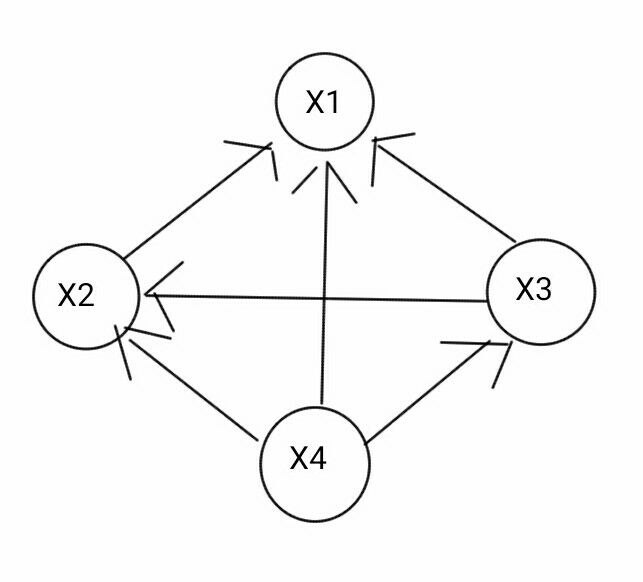
\includegraphics[scale=0.5]{img/grafo1.jpg}

\begin{defn}[Red de Bayes]
\[P(x_1,...,x_n) = \prod_{i=1}^N p(x_i | pa_1)\]

donde $pa_i$ es el conjunto de padres de la variable $x_i$, con $P(x_1|pa_i) = p(x_i)$ en caso de no tener padres la variables $x_i$.

\end{defn}
\obs En caso de ser independientes, las variables no tendrían padres , debido a que el grafo no tendría aristas.


\subsection{Modelo gráfico para Naive-Bayes}
Recordando el problema de las lentillas:
\[P(d|e,l,p) = \frac{P(e,l,p|d)·P(d)}{P(e,l,p)}\]

Con la regla de la cadena:

\[
P(e,l,p|d)·P(d) = P(e,l,p,d) = P(e,l,p|d)·P(d) = P(e|d)P(l|d)P(p|d)P(d)
\]

El grafo correspondiente a este caso:


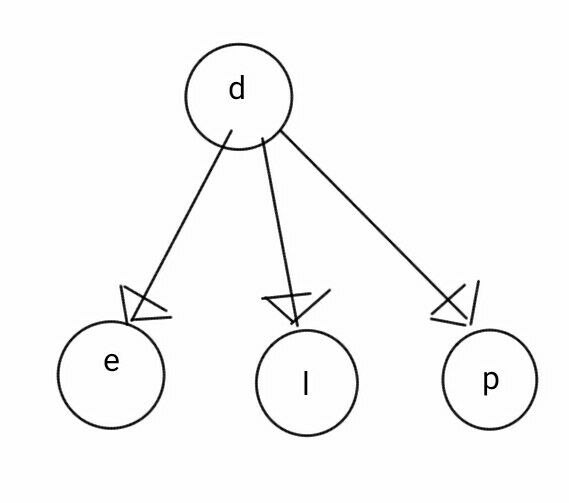
\includegraphics[scale=0.5]{img/grafo2.jpg}

¿Y si este grafo nos parece muy sencillo? Podemos suponer que la edad influye en el astigmatismo, asique añadimos una arista al grafo, y escribimos la fórmula:

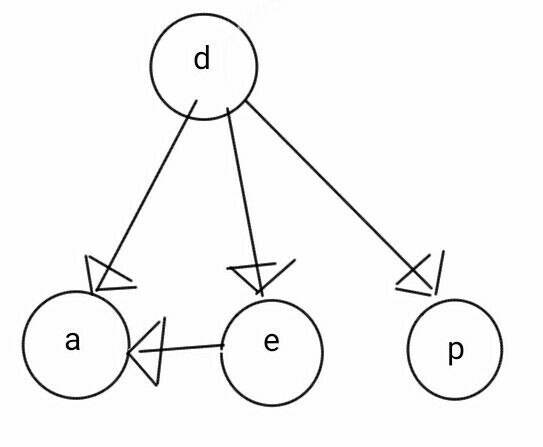
\includegraphics[scale=0.5]{img/grafo3.jpg}

\[
P(d|a,e,p) = \frac{P(d,a,e,p)}{P(a,e,p)} = 
\]

Vamos a descomponer $P(d,a,e,p)$ utilizando el grafo. 

\begin{itemize}
	\item $d$ no depende de nadie, es huérfano sin padres.
	\item $e$ depende de $d$.
	\item $a$ depende de 2 cosas, con lo que $P(a|e,d)$.
	\item ...
\end{itemize}

Con esta información, obtenemos:

\[
P(d|a,e,p) = \frac{P(d,a,e,p)}{P(a,e,p)} =  \frac{P(a|e,d)P(e|d)P(p|d)P(d)}{P(e,a,p)}
\]

Seguimos el próximo día.


Vamos a ver los posibles diagnósticos:

\[
P(d=n|e=j,p=na=s) = \frac{P(a=s|d=n,e=j)P(e=j|d=n)P(p=n|d=n)P(d=n)}{P(...)} = 
\]
\[
= \frac{\frac{2}{4}\frac{4}{15}\frac{3}{15}\frac{15}{24}}{P(...)} = ... = 17\%
\]
\[
P(d=d|e=j,p=na=s) = \frac{\frac{2}{2}\frac{2}{4}\frac{4}{4}\frac{4}{24}}{P(...))} = ... = 83\%
\]
\[
P(d=b|e=j,p=na=s) = ... = 0
\]


\section{Vecinos próximos}

\subsection{Introducción y motivación del método}
Hasta ahora la verosimilitud la hemos calculado de diferentes maneras:

\begin{itemize}
 	\item[Discretos] Con frecuencias 
 	\item[Continuos]  Discretizando y usando frecuencias (histograma). Esta estimación es no paramétrica y la probabilidad de que un punto caiga en una caja es el número de puntos en esa caja dividido del total.
 	\item[] Estimando la densidad de probabilidad con una normal. La estimación es paramétrica y se calcula utilizando la integral de la función de densidad, es decir:
 	\[P(1.4 \leq x < 1.5) = \int_{1.4}^{1.5}P df(x)dx\]
 \end{itemize} 

 ¿Qué podemos hacer para estimar paramétricamente una muestra como la siguiente?

\begin{center}
 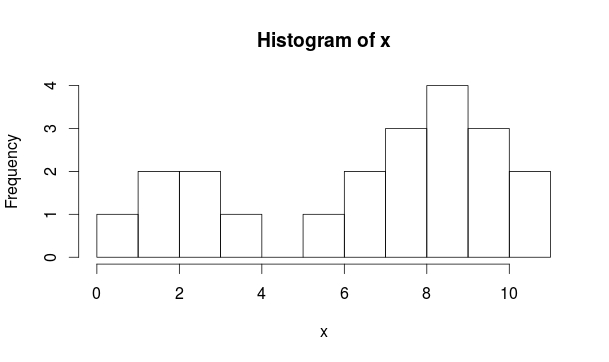
\includegraphics[scale=0.4]{img/histogramaCenas.jpeg}
\end{center}
Aquí vemos claramente que no podemos estimar utilizando una normal, ya que ni se le parece. Podríamos tomar 2 normales, o tendríamos que intentar generalizar la estimación por histograma a $D$ dimensiones.


En el caso de estimar generalizando el histograma, tendríamos $P(x∈R) = \frac{K}{N}$, donde $K$ es el número de puntos en la región y $N$ es el número total de datos.


Si intentamos exportar este modelo a más dimensiones, generalizar la estimación por histograma, necesitamos muchos más datos de los que podemos obtener para estimar así, debido a la \textbf{MALDICIÓN DE LA DIMENSIONALIDAD}. 

Para que la estimación generalizada por histograma sea una buena estimación, tenemos que tener el espacio suficientemente cubierto de puntos, es decir $n$ tiene que ser más grande cuanto mayor es la dimensión.

Si tenemos $R$ suficientemente pequeña, podemos intentar estimarlo con integrales: \[P(\bar{x}∈R) = \int_R Pdf(\bar{x})d\bar{x} \simeq pdf(\bar{x})·V\]
Donde $V$ es el volumen de $R$.

Igualando, obtenemos 

\[
P(\bar{x}∈R) = \frac{K}{N} = pdf(\bar{x})·V \implies pdf(\bar{x}) = \frac{K}{NV}
\]

Esta última fórmula se puede usar de 2 formas:

\begin{itemize}
	\item Si fijamos $K$ y obtenemos el $V$ necesario paar incluir $K$ puntos, clasificamos por el algoritmo de vecinos próximos.
	\item Si fijamos $V$ y calculamos $K$ obtenemos métodos de núcleos (SVM) que son los más eficientes que hay y que no vamos a ver.
\end{itemize}

\begin{defn}[Vecinos próximos]
Fijamos K (el número de vecinos)

Se calcula una esfera alrededor del punto de interés hasta que incluya $K$ puntos.
\end{defn}

\begin{example}
Tenemos 2 clases, cuadrados azules y triángulos verdes. La línea continua corresponde a $K=3$, ya que hemos agrandado la esfera hasta incluir 3 puntos.

\begin{center}
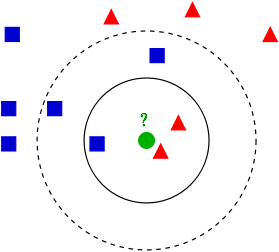
\includegraphics[scale=0.7]{img/VecinosProximos.png}
\end{center}

¿Y cómo asignar la clase? Vamos a ir poco a poco:

\begin{itemize}
	\item \textbf{Verosimilitud} $P(\gor{x} | Clase) = \frac{K_c}{N_cV}$
	\item \textbf{Priori} $P(Clase) = \frac{N_c}{N}$
	\item \textbf{Evidencia} $P(\gor{x}) = \frac{K}{NV}$
\end{itemize}

Con estos datos podemos calcular la probabilidad a posteriori:

\[
P(Clase | \gor{x}) = \frac{...}{...} = \text{ se cancela todo ... } = \frac{K_c}{K}
\]

Con $K=3$ puntos, la clase asignada (a priori) sería ``triángulo rojo'', ya que es la clase con mayor probabilidad a posteriori $\left( \frac{2}{3} \right)$. 

En cambio, si tomamos $K=5$ (la linea discontinua), asignaríamos (a priori) la clase ``cuadrado azul'', ya que es la clase mayoritaria e la esfera.

\end{example}

\subsection{Regla de clasificación $K-NN$}

\paragraph{Algoritmo}
\subparagraph*{Entrenamiento:} Guardar los datos de entrenamiento.
\subparagraph*{Clasificar:} 
\begin{enumerate}
	\item Por cada ejemplo $\gor{z}$ en entrenamiento se calcula la distancia de $\gor{z}$ a $\gor{x}$ usando la métrica.
	\item Se seleccionan los $K$ más cercanos.
	\item Se devuelve la clase más común en esos $K$
\end{enumerate}
\paragraph{Complejidad: } $O(N·\#\{\text{ atributos }\})$

\subsection{Problemas de K-NN}

\subsubsection{Normalizar}
Los cambios de unidades pueden afectar a la clasificación, con lo que necesitamos \textbf{normalizar los datos}. Normalizamos los datos normalizando, es decir, $ y = \frac{x - µ}{σ} ∀x$ y trabajamos con los $y$.


\begin{defn}[Poligonos de Thiessen]
Tomamos un punto y haciendo mediatrices con los $K$ vecinos cercanos, creamos los polígonos.
\begin{center}
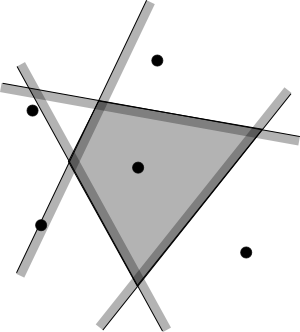
\includegraphics[scale=0.5]{img/Voronoi_cell.png}
\end{center}

A la hora de clasificar, comprobamos a qué polígono pertenece.
\end{defn}

\subsubsection{Elección de $K$}

\paragraph{Selección de $K$ óptimo:}
\begin{itemize}
	\item Calcular distancias entre todos los pares de puntos.
	\item Para cada ejemplo:
		\subitem Se ordena el resto de eemplos por distancias.p
		\subitem Se hacen tantas clasificaciones como valores de  $K$ estemos evaluando.
	\item Se calcula el error y nos quedamos con el que menor error tenga.
\end{itemize}

\section{Clasificadores lineales}

Son aquellos que dan lugar a fronteras de decisión lineales. En 2 dimensíones es una recta, en $n$ dimensiones es un hiperplano.

\begin{defn}[Clasificador lineal]
Sea $h$ un clasificador lineal:

\[h(\vec{x}) = \left\{ \begin{array}{cc}
 c_1 & \pesc{\vec{ω},\vec{x}} + ω_0 > 0\\ 
 c_2 & \pesc{\vec{ω},\vec{x}} + ω_0 < 0\\ 
 \end{array} \right.\]

Llamamos \concept{Frontera} al hiperplano $\pesc{\vec{ω},\vec{x}} + ω_0$.

\end{defn}

\begin{example}
Vamos a construir la frontera de manera genérica. Para ello, tenemos:

\[
\pesc{\vec{ω}\vec{x}} + ω_0 = 0 \to |\vec{x}|\cos(α) = \frac{-ω_0}{|\vec{ω}|}
\]

\begin{center}
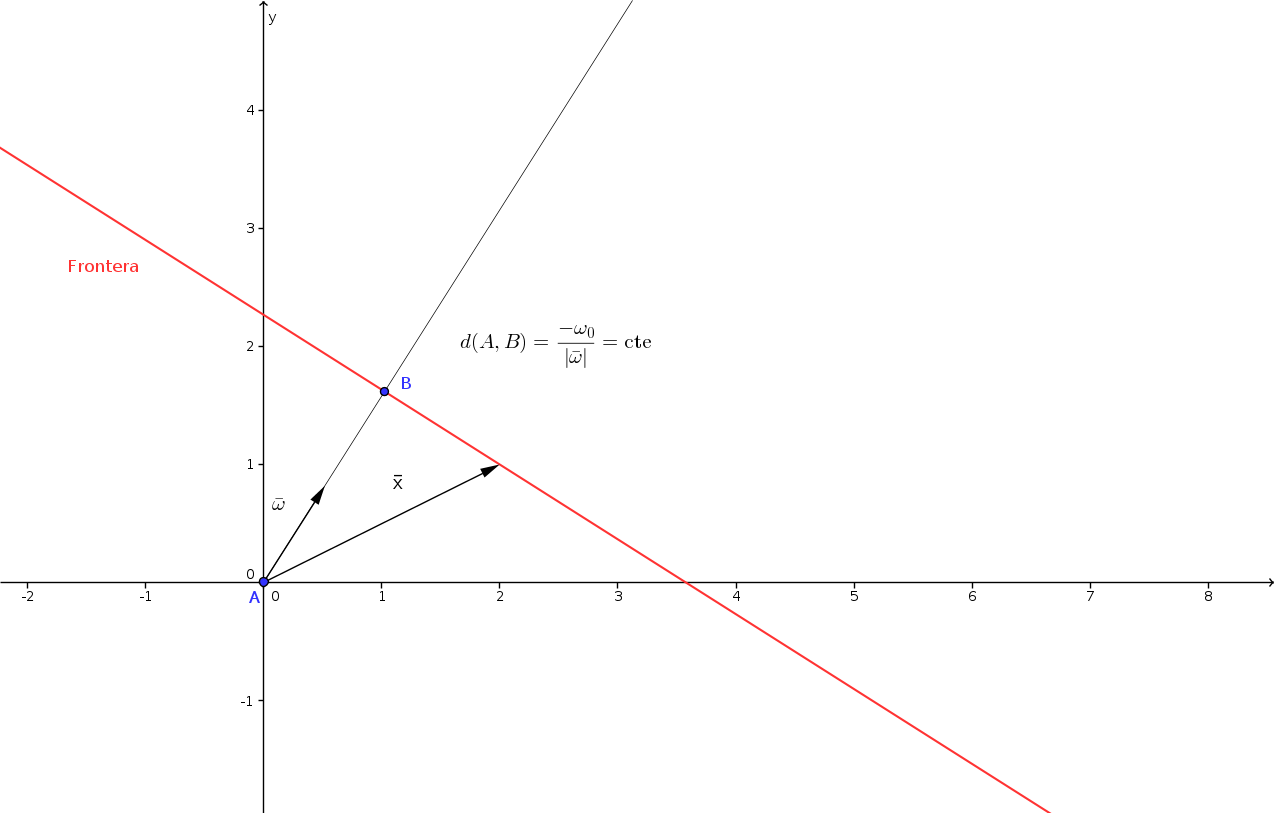
\includegraphics[scale=1.4]{img/ClasificadorLineal.png}
\end{center}
\end{example}

Veamos como surgen las fronteras lineales de forma ``natural'' haciendo suposiciones sencillas sobre la forma funcional de los datos.

\begin{defn}[Función sigmoidal]

Consideramos un problema de dos clases $C_1,C_2$. Podemos escribir la probabilidad a posterior:

\[
P(C_1 | \vec{x}) = \frac{P(\vec{x}|C_1)P(C_1)}{P(\vec{x})} = \frac{P(\vec{x}|C_1)P(C_1)}{\sum P(\vec{x}|C_i)P(C_i)}\]
Dividimos numerador y denoiador por $P(\vec{x}|C_1)(C_1)$
\[
\frac{1}{1+c} = \frac{1}{1+e^{-a}} = σ(a)
\]
donde $a = ln(c)$ y $c=\displaystyle\frac{P(\vec{x}|C_1)P(C_1)}{P(\vec{x}|C_2)P(C_2)}$

¿Qué hemos ganado con esto? Hemos reescrito Bayes como una \href{https://es.wikipedia.org/wiki/Funci\%C3\%B3n\_sigmoide}{sigmoidal}.

Esto permite clasificar de la siguiente manera:

\[P(\vec{x} | C_1) P (C_1) > P(\vec{x} | C_2) P (C_2) \implies \text{ elegimos } C_1\]

Esto es equivalente a ``si a > 0, entonces elegimos $C_1$, sino, elegimos $C_2$''
\end{defn}

Suponemos que la veroimilitud sigue una distribución normal en $n$ dimensiones, siendo $\bm{µ_k}$ el vector de medias y $\Sigma$ la matriz de covarianzas. Todos los productos entre vectores son productos escalares. Ante cualquier tipo de duda (de que no cuadran las dimensiones, etc...) aplicar el producto escalar.

\[
p(\vec{x}|C_{x} = \frac{1}{(2π)^{\frac{n}{2}}}\frac{1}{|\Sigma|^{\frac{1}{2}}} \exp \left\{  \frac{-1}{2} (\vec{x} - \bm{µ_k}) \Sigma_k^{-1} (\vec{x} - \bm{µ_k}) \right\} 
\]


\subsection{Frontera de decisión con hiperplano (2 clases)}
Suponiendo:

\begin{itemize}
	\item  tenemos 2 clases.
	\item $\Sigma_1 = \Sigma_2 = I$
\end{itemize}

Vamos a construir la frontera de decisión con hiperplano para 2 clases:

\[
a = \ln\left( \frac{P(\vec{x}|C_1)P(C_1)}{P(\vec{x}|C_2)P(C_2)}\right) = \ln \left\{ \exp \left\{ \frac{\vec{x}-\bm{µ_1}}{2} - \frac{\vec{x} - \bm{µ_2}}{2} \right\} \frac{P(C_1)}{P(C_2)}\right\} = 
\]
\[
= \left( \frac{(\vec{x} - \bm{µ_2})^2}{2} - \frac{(\vec{x} - \bm{µ_2})^2}{2}\right) + \ln \frac{P(C_1)}{P(C_2)} = 0
\]
Si $P(C_1) = P(C_2)$, tenemos:
\[
\left( \frac{(\vec{x} - \bm{µ_2})^2}{2} - \frac{(\vec{x} - \bm{µ_2})^2}{2}\right) = 0
\]
Si $(\vec{x} - \bm{µ_2})^2 > (\vec{x} - \bm{µ_1})^2 \implies C_1$. ¿Porué $C_1$? Porque estamos más lejos de la media $\bm{µ_2}$ que de la media $\bm{µ_1}$. Es como vecinos próximos si sólo tuvieramos 2 vecinos, la media de 1 y la media del otro.

Si por el contrario, $P(C_1) ≠ P(C_2)$, tenemos: 

\[
\frac{\vec{x}^2 + \vec{\mu}_2^2 - 2\vec{x}\vec{\mu}_2}{2} - \frac{\vec{x}^2 + \vec{\mu}_1^2 - 2\vec{x}\vec{\mu}_1}{2} + \ln\frac{P(C_1)}{P(C_2)} = 
\]
\begin{equation}
= (\vec{\mu}_1 - \vec{\mu}_2) \vec{x} + \frac{1}{2} (\vec{\mu}_2^2 - \vec{\mu}_1^2) + \ln\frac{P(C_1)}{P(C_2)} = 0
\end{equation}
Esto es un hiperplano que utilizaremos como frontera de decisión. 

\begin{framed}
En este caso, tenemos $\vec{ω} = \bm{µ_1} - \bm{µ_2}$ y $\vec{ω_0} = \frac{1}{2}(µ_2^2 - µ_1^2) + \ln \frac{P(C_1)}{P(C_2)}$

Es decir, el hiperplano será:

\[
\pesc{ω,\vx} + ω_0 = 0 \implies \pesc{(\bm{µ_1} - \bm{µ_2}),\vx} + \frac{1}{2}(µ_2^2 - µ_1^2) + \ln \frac{P(C_1)}{P(C_2)}
\]
\end{framed}


\subsubsection{Ampliamos las suposiciones I}

\begin{itemize}
	\item 2 clases
	\item Verosimilitud normal en $D-$dimension con $Σ_{1} = Σ_2 = Σ$
\end{itemize}

Entonces, la frontera de decisión:

\[
a = 0 = \ln\left(\frac{P(\vx|C_1)P(C_1)}{P(\vx|C_2)P(C_2)} \right)
\]

Desarrollando igual que antes, obtenemos que la frontera de decisión óptima es un hiperplano:

\[ω = Σ^{-1}(\bm{µ_1} - \bm{µ_2})\]
\[ω_0 = \frac{1}{2} \bm{µ_1}Σ\bm{µ_1} + \frac{1}{2} \bm{µ_2}Σ\bm{µ_2} + \ln \left( \frac{P(C_1)}{P(C_2)}\right)\]


Ahora vamos a obtener los parámetros de las gausianas por máxima verosimilitud, es decir: $\max_i\{P(D|H_i)\}$

Tenemos: 
\begin{align*}
D &= \{(\vx_i,y_i) i=1,...,N_{train}\}\\
H &= \{\bm{µ_1},\bm{µ_2},Σ\}
\end{align*}

Vamos a ello:

\[
P(D|H) = P(\{\vx_i,y_i\} | \bm{µ}_1\bm{µ_2}Σ) = \prod_i^{N_{train}} P(\vx_iy_i | \bm{µ_1},\bm{µ_2},Σ)
\]

Ahora aplicamos el logaritmo, derivamos e igualamos a 0.

Este es el enfoque de regresión logística.

\textcolor{blue}{Si te parece que queda colgado este final, a mi no me preguntes porque ha sido así de literal en clase}.

\section{Regresión logística}

Aunque la regresión logística se llame regresión logistica, no es un método de regresión. Es un método de clasificador.

La probabilidad a posteriori de $C_1$ es:
\[
P(C_1 | \vx) = σ(a) = σ(\pesc{\bm{ω},\vx} + ω_0)
\]
¿Cuántos parámetros habría que estimar en $\bm{µ_1,µ_2},Σ$? Sabiendo que $P(\vx | C_i) = N(\bm{µ_i},Σ) $

Tenemos  $2D$ por $\bm{µ_i}$ más, $\frac{D(DH)}{2}$ por $Σ$ y 2 ($P(C_i)$), es decir demasiados.

En cambio, utilizando la probabilidad a posteriori de $C_i$, sólo hay que estimar $\bm{ω},ω_0$, es decir, $D+1$ parámetro.

\paragraph{Notación:} Para simplificar, vamos a escribir:
\[\bm{ω}_{new} = (ω_0, \bm{ω})\]
\[\bm{x}_{new} = (1, \bm{x})\]
¿Qué hemos ganado con esto? Algo más de compacidad, ya que $P(C_1 | \vx) = σ(\pesc{\bm{ω}_{new},\vx_{new}})$

\begin{example}
Disponemos de $N$ ejemplos.

\[
D = \{ (\vx_i,t_i) i=1,...,N\}
\]

donde $t_i = \left\{ \begin{array}{cc} 1 & x_i ∈ C_1 \\ 0 & x_i ∈ C_2\end{array}\right.$

En regresión logística, 
\begin{itemize}
	\item $H = \bm{ω}$
	\item $D = t_1,...,t_N$
	\item $I = \bm{x_1},...,\bm{x_N}$
\end{itemize}


\textbf{Objetivo:} maximizar por $MV$ para encontrar los valores de $\bm{ω}$.

La verosimilitud es:

\[
P(t_1,...,t_N | \bm{ω},\bm{x}_1,...,\vx_N) = \prod^N P(t_i | \bm{ω},\vx_i)
\]

Con la codificación de $t_i$, podemos escribir:

\[
P(t_i | \bm{ω},\vx_i) = σ\left(\pesc{\bm{ω},\vx_i}\right)^{t_i}·\left(1-σ(\pesc{\bm{ω},\vx_i})\right)^{(1-t_i)}
\]

Juntando y llamando a $σ_i = σ(\bm{ω},\vx_i)$:

\[
= ... = \prod^N σ_i^{t_i} (1-σ_i)^{(1-t_i)}
\]

Primero aplicamos el $-\ln$ para simplificar el cálculo y derivamos:

...
...
...

\paragraph{Conclusión:}

10 minutos después sigue haciendo cuentas.


\paragraph{En la clase siguiente} se tomó la decisión de mejor optimizar ejemplo a ejemplo.

\end{example}


\begin{example}
Sea $\vec{ω} = \{ -1,\frac{1}{3},\frac{2}{3} \}$ y queremos clasificar los datos $x_1 = (0,0)$ y $x_2 = (3,1.5)$. Los coeficientes se han calculado tomando como clase de referencia o clase principal $C_1$.


\begin{itemize}
	\item[$x_1$] \[\pesc{\vec{ω},(1,x_1)} = \pesc{\left(-1,\frac{1}{3},\frac{2}{3}\right), (1,0,0)} = -1 \]

	Y ahora aplicamos la sigmoidal:

	\[P(C_1 | x_1) = \frac{1}{1+e^{-(-1)}} = 0.27\]

	\subitem Comentamos que $P(C_2 | x_1) = 1 - P(C_1 | x_1)$

	\item[$x_2$] \[\pesc{\vec{ω} , \left(1,3,1.5\right)} = ... = 1 \]

	 Y ahora aplicamos la sigmoidal:

	\[P(C_1 | x_2) = \frac{1}{1+e^{-1}} = 0.73\]
\end{itemize}


\obs Es interesante ver que son los complementarios. ¿A qué se debe esto? A que están a la misma distancia de la recta frontera.

\end{example}

\subsection{Algoritmo de la regresión logística}

Para aumentar la verosimilitud de $t_i$ del ejemplo $\vec{x_i}$ hay que mover la recta $\vec{ω}$ en sentido opuesto al gradiente $(σ_i - t_i)\vec{x_i}$ y proporcional a una constante de aprendizaje $\eta = \vec{ω} + \vec{ω} - \eta (σ_i - t_i)\vec{x_i}$

\paragraph*{Algoritmo}

Definimos 2 parámetros: $\eta$ y $epocas$ (estos parámetros se darán como argumento)

\begin{itemize}
	\item[1] Generamos un $\vec{ω}$ aleatorio con componentes entre $-1$ y $1$.
	\item[2] for (ie=1;ie<epocas;ie++) for(i = 1; i < N; i++)
	\subitem[2.1] calculamos $σ_i = σ(\pesc{\vec{ω},\vec{x}_i})$
	\subitem[2.2] Actualizamos $\vec{ω} = \vec{ω} - \eta (σ_i - t_i)\vec{x_i}$
	\item[3] return $\vec{ω}$
\end{itemize}

El coste del entrenamiento del algorimo es $O(epocas·N·\#atributos$


\begin{example}
\begin{center}
\begin{tabular}{cccc}
$x_1$ & $x_2$ & t & \\
0&0&0&$C_2$\\
1&1&0&$C_2$\\
0&1&0&$C_2$\\
1&1&1&$C_1$
\end{tabular}
\end{center}

Tomamos $\eta = 1$ y arbitrariamente $\vec{ω} = \{ -0.3,0,0.4 \}$

La frontera de decisión entonces es: \[-0.3 + 0x_1 + 0.4x_2 = 0 \to x_w = \frac{0.3}{0.4}\]

Ejemplo: $\vec{x} = (1,0,0)$

\[ \pesc{\vec{ω},\vec{x}} = -0.3 \]
\[ σ(-0.3) = \frac{1}{1+e^{-(-0.3)}} = 0.43\]

Está bien claisificado, ya que da $C_2$ (la principal es $C_1$).

\[
\vec{ω} = \vec{ω} - \eta (σ - t)\vec{x} = (-0.3,0,0.4) -1(0.43-0)(1,0,0) = (0.73,0,0.4)
\]


Vamos a hacer otra iteración del bucle. Ahora toca $\vec{x} = (1,1,0)$:

\[\pesc{\vec{ω},\vec{x}} = 0.73\]
...
\[
\vec{ω} = (-1.06,-0.33,-0.4)
\]

\end{example}


%% Apéndices (ejercicios, exámenes)
\appendix


\chapter{Ejercicios}
% -*- root: ../AprendizajeAutomatico.tex -*-

\section{Hoja 1}

\begin{problem}[1]

Un taxi golpea a una persona de noche y huye. En la ciudad operan dos compañías de taxis. Una verde y otra azul. El 85\% de los taxis son verdes. 

\ppart
¿De qué color es más probable que sea el taxi?

\ppart
Un testigo dice que es azul con fiabilidad del 80\%

\solution
\paragraph{Notación} H de hipótesis, D de Datos e I de información.

\spart
Se deja como ejercicio para el lector experimentado.

\spart
P(H=verde) = 85\%
P(H=azul) = 15\%

\[
P\left( H=azul | D=azul, I \right) = \frac{P(D=a|H=a,I)·P(H=A|I)}{P(D=a|I)}
\]

Para calcularlo, necesitamos saber la probabilidad con la que el testigo dice que un taxi es azul.\footnote{Suponemos que el testigo se equivoca igual de azul a verde que de verde a azul}
\[
P(D=a|I) = P(D=a|H=a)·P(H=a) + P(D=verde | H=v) · P(H=v) = 0.8·0.15 + 0.2·0.85 = 0.29
\]

Con esto ya tenemos:

\[
 P\left( H=azul | D=azul, I \right) = \frac{0.8·0.15}{0.29} = 0.41
\]

Por el contrario, la probabilidad de que el taxi sea verde (utilizando la información del testigo) es de un 0.59.

\paragraph{Notación} Observamos que todas las probabilidades son condicionadas a I, que no influye en nada y omitiremos cuando no sea influyente
\end{problem}


\begin{problem}[4]
Tenemos 2 bolsas. La bolsa A tiene 2 bolas negras y 3 blancas. La bolsa B tiene 3 bolas negras y 2 blancas.

\ppart Se elige una de las bolsas al azar, y escogemos al azar una bola. ¿Cuál es la probabilidad de que sea negra?

\ppart Habiendo extraido una bola negra. ¿Cuál es la bolsa más probable?
\solution

\spart 
\[
P(negra) = P(A,negra) + P(B,negra) = P(negra|A,I)·P(A) + P(negra|B,I)·P(B)\]
\[
P(negra) = 0.4*0.5+0.6*0.5 = 0.5
\]
\spart La intuición nos dice que será de la bolsa B, ya que esta tiene más bolas negras, y las 2 bolsas son equiprobables.

Vamos a justificarlo matemáticamente:

P(H=A) = 50\%

D=negra

\[
P(A|D=negra) = \frac{P(negra|A)·P(A)}{P(negra)}
\]




\end{problem}
\printindex

\end{document}
